Although Canada is a large country, many areas are uninhabited, and most of the population lives near the southern border. The TransCanada Highway, completed in 1962, connects the people living in this strip of land, from St. John's in the East to Victoria in the West, a distance of 7 821 km.

Canadians like hockey. After a hockey game, thousands of fans get in their cars and
drive home from the game, causing heavy congestion on the roads. A wealthy
entrepreneur wants to buy a hockey team and build a new hockey arena. Your task is
to help him select a location for the arena to minimize the traffic congestion after a
hockey game.

The country is organized into cities connected by a network of roads. All roads are bidirectional, and there is exactly one route connecting any pair of cities. A route connecting the cities $c_0$ and $c_k$ is a sequence of distinct cities $c_0, \cdots, c_k$ such that there is a road from $c_{i-1}$ to $c_i$ for each $i$. The new arena
must be built in one of the cities, which we will call the arena city. After a hockey game, all of the hockey fans travel from the arena city to their home city, except those who already live in the arena city. The amount of congestion on each road is proportional to the number of hockey fans that travel along the road. You must locate the arena city such that the amount of congestion on the most congested road is as small as possible. If there are several equally good locations, you may choose any one.

\begin{tabular}{ccc}
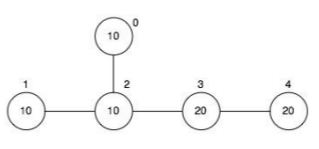
\includegraphics[scale=0.45]{traffic1.png} &
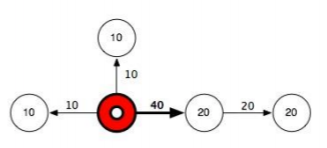
\includegraphics[scale=0.45]{traffic2.png} &
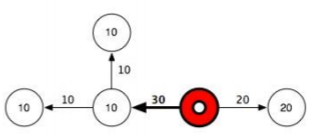
\includegraphics[scale=0.45]{traffic3.png}
\end{tabular}


You are to implement a procedure \t{LocateCentre(N,P,S,D)}. $N$ is a positive integer,
the number of cities. The cities are numbered from $0$ to $N-1$. $P$ is an array of $N$
positive integers; for each $i$, $P[i]$ is the number of hockey fans living in the city
numbered $i$. The total number of hockey fans in all the cities will be at most
$2\,000\,000\,000$. $S$ and $D$ are arrays of $N-1$ integers each, specifying the locations of  roads. For each $i$, there is a road connecting the two cities whose numbers are $S[i]$ and $D[i]$. The procedure must return an integer, the number of the city that should be the arena city.


As an example, consider the network of five cities in the left diagram on the top,
where cities $0$, $1$ and $2$ contain $10$ hockey fans each, and cities $3$ and $4$ contain $20$
hockey fans each. The middle diagram shows the congestions when the new arena is
in city $2$, the worst congestion being $40$ on the thicker arrow. The right diagram
shows the congestions when the new arena is in city $3$, the worst congestion being $30$
on the thicker arrow. Therefore, city $3$ would be a better location for the arena than
city $2$. The data for this example are in 3-rd example test.